\documentclass[12pt]{article}
\usepackage[arabic]{babel}
\usepackage[utf8]{inputenc}
\usepackage{amssymb}
\usepackage{geometry}
\usepackage{graphicx}
\usepackage{wrapfig}
\usepackage{amsmath}
\usepackage{xcolor}
\usepackage{polyglossia}
\usepackage{tikz}
\usetikzlibrary{positioning, shapes}

% Font and layout settings
\setdefaultlanguage{arabic}
\setotherlanguage{english}
\newfontfamily\arabicfont[Script=Arabic,Scale=1.2]{Amiri}
\geometry{top=2cm, bottom=2cm, left=2cm, right=2cm}

% Colors
\definecolor{titleColor}{HTML}{800000} % Maroon for titles
\definecolor{sectionColor}{HTML}{4682B4} % SteelBlue for sections
\definecolor{textHighlight}{HTML}{DAA520} % Goldenrod for highlights
\definecolor{backgroundColor}{HTML}{F0F8FF} % AliceBlue background
\definecolor{emphasisColor}{HTML}{228B22} % ForestGreen for emphasis

% Page styling
\pagecolor{backgroundColor}
\color{black}

\begin{document}

\begin{center}
    {\Huge\textbf{\textcolor{titleColor}{السودان: الحرب، السلام، الاستقرار، والازدهار}}} \\
    \vspace{0.5cm}
    \textbf{\textcolor{emphasisColor}{بابكر عثمان}} \\
    \vspace{0.2cm}
    \today
\end{center}

\begin{wrapfigure}{r}{0.9\textwidth}
    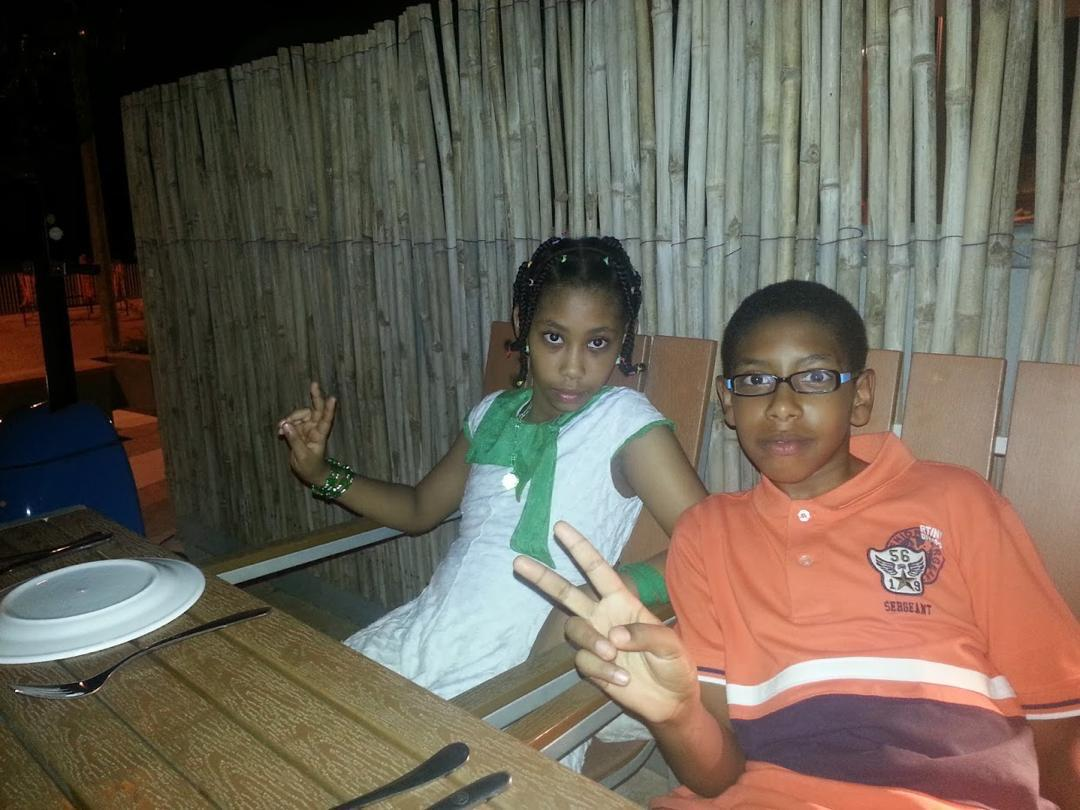
\includegraphics[width=0.9\textwidth]{d9.jpg}
    \caption{\textcolor{sectionColor}{أطفال الماضي أجداد اليوم}}
\end{wrapfigure}

\end{document}



2025-09-04
2025-10-02 
